\documentclass[pdf,genome,nocolorBG,slideColor,noaccumulate,nototal]{prosper}

\usepackage{pstricks}
\usepackage{pst-grad}

\title{Cluster Workshop}

\Logo{
\includegraphics[width=.9cm]{genlogo.eps}}

\begin{document}

\begin{slide}{Cluster Workshop}
\begin{center}
	\rput(-.5,-2.75){
\includegraphics{genbanner.eps}}
\end{center}
\end{slide}

%-----------------

\begin{slide}{Introduction}
``If you were plowing a field, which would you rather use: Two strong oxen 
or 1024 chickens?''

--Seymour Cray
\end{slide}

\overlays{6}{%
\begin{slide}{Introduction}
\begin{itemstep}
	\item What is a cluster?
	\begin{itemize}
		\item A collection of machines that work together
	\end{itemize}
	\item Why use a cluster?
	\begin{itemize}
		\item Chickens are cheaper than oxen
		\item (and easier to feed)
		\item ...but try making 1024 chickens move in the same direction
	\end{itemize}
\end{itemstep}
\end{slide}}

\overlays{3}{%
\begin{slide}{Types of Jobs}
\begin{itemstep}
	\item {\bf interactive}
		A single-part job to be run immediately.
	\item {\bf batch (serial)}
		A single-part job to run in the background
	\item {\bf parallel}
		A job that has been split into multiple parts to run on more than one
		processor. 
\end{itemstep}
\end{slide}}

\overlays{3}{%
\begin{slide}{Types of Jobs}
Parallel cluster jobs can be categorized according to the amount of 
communication required between parts of the job:
\begin{itemstep}
	\item {\bf fine-grained parallel}
			Substantial communication required.
	\item {\bf course-grained parallel}
			Occasional communication required.
	\item {\bf embarrassingly parallel}
			Almost no communication required.
\end{itemstep}
\end{slide}}

\begin{slide}{Types of Jobs}

Even serial jobs that cannot be split up to run in parallel can still benefit
from a cluster environment, for example, by running with different 
sets of input files or parameters simultaneously.
\end{slide}

%-----------------

\overlays{4}{%
\begin{slide}{Cluster Terminology}
\begin{itemstep}
	\item {\bf Node}
		An individual computer in the cluster
	\item {\bf Head Node}
		The main node.  Coordinates scheduling jobs among the nodes. This is 
what you log in to from outside.
	\item {\bf Interconnect}
		The network or networks that connects the nodes together
	\item {\bf MPI}
		{\bf M}essage {\bf P}assing {\bf I}nterface, a protocol used for
		communication between parts of a job.
\end{itemstep}
\end{slide}}

\overlays{3}{%
\begin{slide}{Cluster Storage}
\begin{itemstep}
	\item Home directory
	\item Shared cluster space
	\item Local storage
\end{itemstep}
\end{slide}}

\overlays{3}{%
\begin{slide}{Storage: Home directory}
\begin{itemstep}
	\item Network mounted
	\item Geared towards wide availability, not high performance
	\item Good place for your code, final results
\end{itemstep}
\end{slide}}

\overlays{4}{%
\begin{slide}{Storage: shared}
\begin{itemstep}
	\item Network shared, but only within the cluster
	\item Medium availability, medium performance
	\item Good place for dataset that all nodes need to access
	\item Performance can suffer with many simultaneous accesses
\end{itemstep}
\end{slide}}

\overlays{3}{%
\begin{slide}{Storage: local}
\begin{itemstep}
	\item Not network shared, only available to a single node
	\item Highest performance, but least convenient
	\item Good place for working set
\end{itemstep}
\end{slide}}

\begin{slide}{Anatomy of a Cluster}
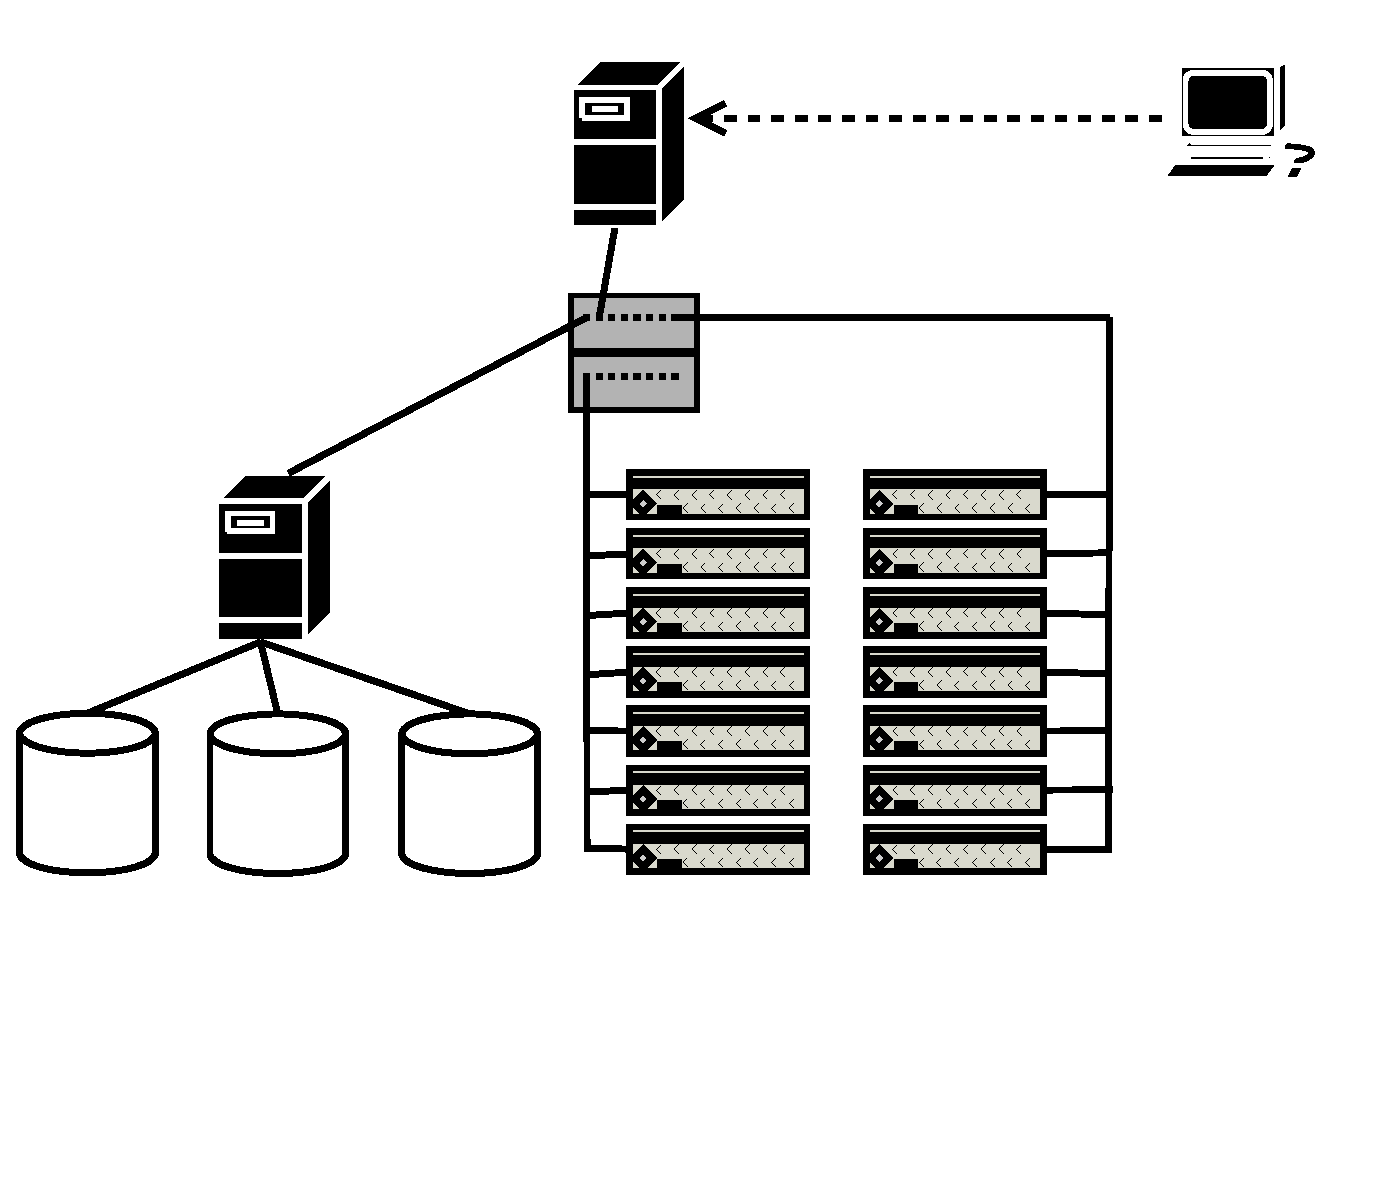
\includegraphics[height=8cm]{cluster_network.eps}
\end{slide}

\overlays{3}{%
\begin{slide}{Accessing the cluster}
\begin{itemstep}
	\item Access using ssh
	\item Transfer files using scp/sftp/rsync
	\item Web interface
\end{itemstep}
\end{slide}}

\overlays{8}{%
\begin{slide}{Data Transfer}
\begin{itemstep}
	\item scp
	\begin{itemize}
		\item {\tiny \tt scp file username@genbeo:}
	\end{itemize}
	\item rsync
	\begin{itemize}
		\item {\tiny \tt rsync -a directory username@genbeo:}
	\end{itemize}
	\item sftp
	\begin{itemize}
		\item ftp-like interface that works over ssh
	\end{itemize}
	\item wget
	\begin{itemize}
		\item client to download files from the web directly to the cluster
	\end{itemize}
\end{itemstep}
\end{slide}}

\begin{slide}{Web Interface}
\begin{center}

\includegraphics[height=6cm]{rocks-web-main.eps}
\end{center}
\end{slide}

\begin{slide}{Cluster Web Interface}
\begin{center}
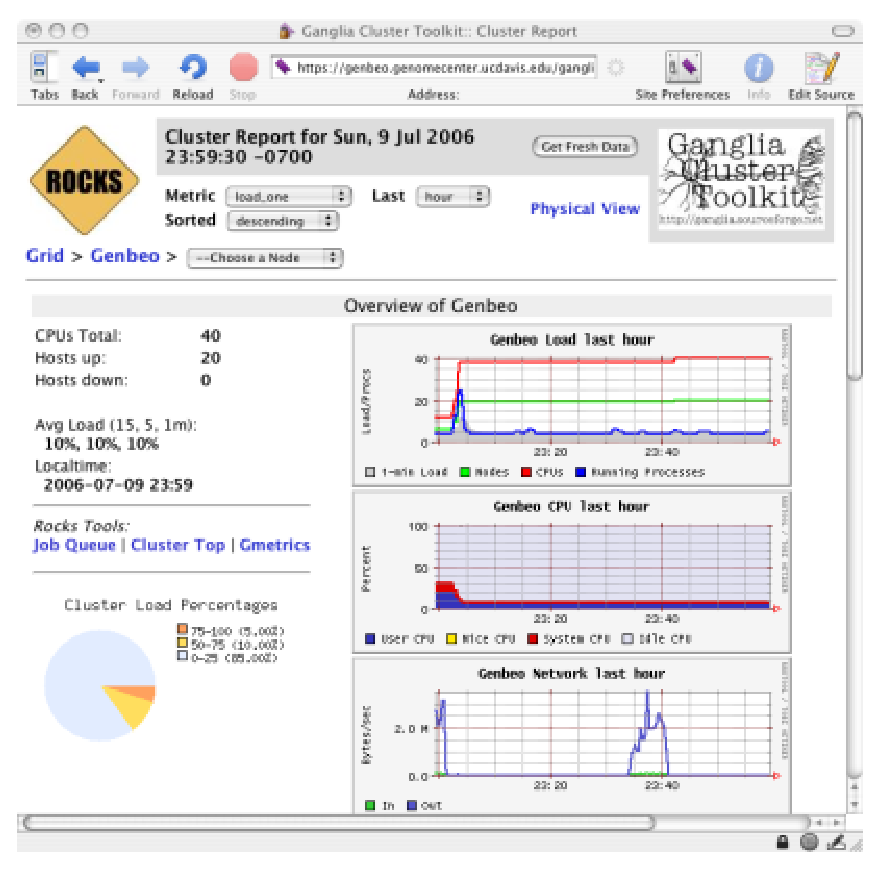
\includegraphics[height=6cm]{rocks-web-report.eps}
\end{center}
\end{slide}

\begin{slide}{Cluster Web Interface}
\begin{center}
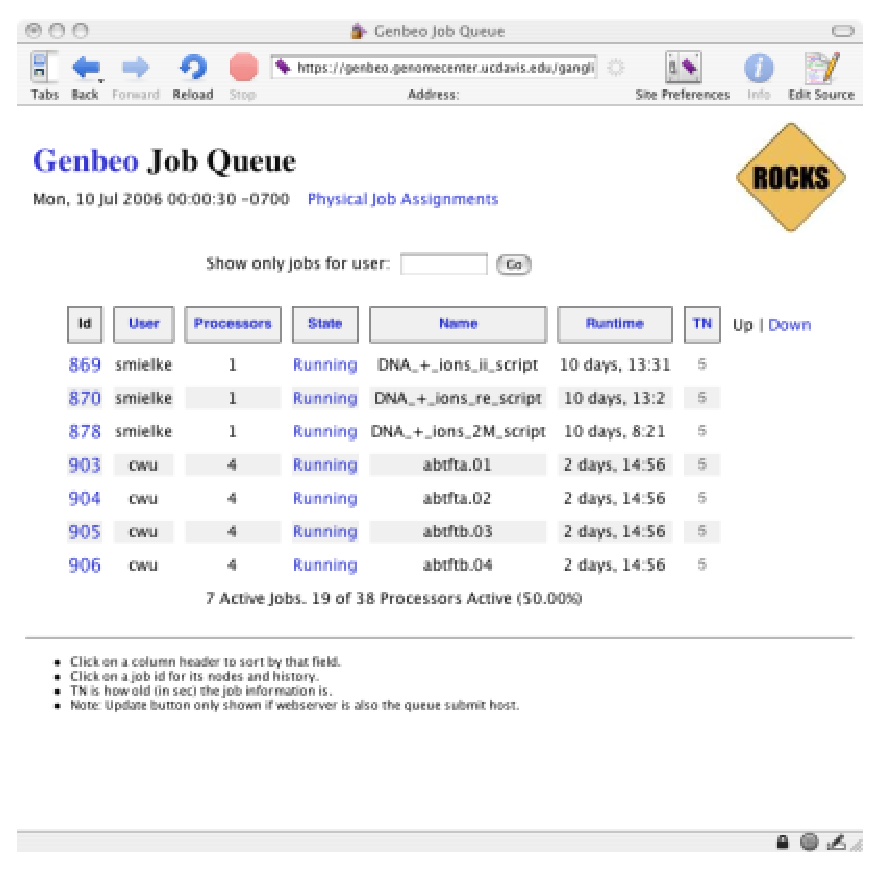
\includegraphics[height=6cm]{rocks-web-jobq.eps}
\end{center}
\end{slide}

\overlays{6}{%
\begin{slide}{Sun Grid Engine}
\begin{itemstep}
	\item What is a batch queue?
	\begin{itemize}
		\item Manage cluster resources
	\end{itemize}
	\item Why use the batch queue?
	\begin{itemize}
		\item Share cluster resources
		\item You don't need to worry about when/where your jobs run
		\item Submit a whole bunch of jobs and go home!
	\end{itemize}
\end{itemstep}
\end{slide}}

\overlays{3}{%
\begin{slide}{The Cluster Caf\'{e} }
You can think of the cluster as a restaurant:
\begin{itemstep}
	\item {\bf Jobs} are parties coming to eat
	\item {\bf Tables} are the nodes of the cluster
	\item Usually the scheduler will try to place each job at its own table,
		but if it's a busy day, you might have to share a table with someone
		you don't know.
\end{itemstep}
\end{slide}}

\overlays{4}{%
\begin{slide}{Slots}
A {\bf slot} is a placeholder where a job or part of a job can run.  In
the Cluster Caf\'{e}, it is a chair at a table.
\begin{itemstep}
	\item A resource allocated to your job.
	\item We define one slot per CPU core
	\item Request number of slots when you submit job
	\item Allocating a slot is only advisory: the scheduler has reserved
		the requested number of slots.
\end{itemstep}
\end{slide}}

\overlays{5}{%
\begin{slide}{Resources}
\fromSlide{1}{%
It is possible to request other resources when you submit your job}

\fromSlide{2}{%
\hskip 1cm $\Rightarrow$``I'd like a table by the window''}
\vskip .5cm
\fromSlide{3}{%
Or even to request a specific node}

\fromSlide{4}{%
\hskip 1cm $\Rightarrow$``I want to sit at table 2. I'll wait.''}
\vskip .5cm
\fromSlide{5}{%
The scheduler will wait to run your job until it can fulfill your
requirements.}
\end{slide}}

\overlays{3}{%
\begin{slide}{Parallel Environment}
A {\bf Parallel Environment} sets up the resources required to run a multi-node
job. 
\begin{itemstep}
	\item Need to use a PE when you want more than one slot
	\item Request desired PE when you submit your job
\end{itemstep}
\fromSlide{3}{%
Tells the scheduler how you'd like the table set}
\end{slide}}

\overlays{3}{%
\begin{slide}{Parallel Environment}
Available PEs:
\begin{itemstep}
	\item mpi
		Sets up environment for LAM MPI
	\item mpich
		Sets up environment for mpich
	\item serial/threaded
		Makes sure all slots are on the same node, does not set up any inter-node
		communication environment.
\end{itemstep}
\end{slide}}

\overlays{3}{%
\begin{slide}{Job Arrays}
\begin{itemstep}
	\item Run the same job multiple times
	\item submit/manage as a single job
	\item Ideal for running the same program repeatedly with different
         input files or parameters
\end{itemstep}
\end{slide}}

\begin{slide}{Queue example}
Three jobs:
\begin{itemize}
	\item A parallel job using 6 slots
	\item A job array of 3 jobs, using one slot each
	\item A parallel job using 4 slots
\end{itemize}
\end{slide}

\overlays{9}{%
\begin{slide}{Queue example}
\begin{tabular}{ccc}
\begin{tabular}{|c|c|}
\hline
Job & Slots \\
\hline
\untilSlide{4}{\green $A$} 	& \untilSlide{4}{6} \\
\hline
\untilSlide{6}{\red $B_1$}		& \untilSlide{6}{1} \\
\untilSlide{7}{\red $B_2$}		& \untilSlide{7}{1} \\
\untilSlide{9}{\red $B_3$}		& \untilSlide{9}{1} \\
\hline
\untilSlide{9}{\blue $C$}		& \untilSlide{9}{4} \\
\hline
\end{tabular} 
&
\begin{tabular}{|c|c|}
\hline
\onlySlide*{1}{\hspace{.38cm}}%
\onlySlide*{2}{\green $A$}%
\onlySlide*{3}{\green $A$}%
\onlySlide*{4}{\green $A$}%
\onlySlide*{5}{\hspace{.38cm}}%
\onlySlide*{6}{\hspace{.38cm}}%
\onlySlide*{7}{\hspace{.38cm}}%
\onlySlide*{8}{\hspace{.38cm}}%
\onlySlide*{9}{\hspace{.38cm}}%
& 
\onlySlide*{1}{\hspace{.38cm}}%
\onlySlide*{2}{\green $A$}%
\onlySlide*{3}{\green $A$}%
\onlySlide*{4}{\green $A$}%
\onlySlide*{5}{\hspace{.38cm}}%
\\
\hline
\onlySlide*{2}{\green $A$}%
\onlySlide*{3}{\green $A$}%
\onlySlide*{4}{\green $A$}%
&
\onlySlide*{2}{\green $A$}%
\onlySlide*{3}{\green $A$}%
\onlySlide*{4}{\green $A$}%
\onlySlide*{6}{\red $B_3$}%
\onlySlide*{7}{\red $B_3$}%
\onlySlide*{8}{\red $B_3$}%
\onlySlide*{9}{\red $B_3$}%
\\
\hline
\end{tabular} 
&
\begin{tabular}{|c|c|}
\hline
\onlySlide*{1}{\hspace{.38cm}}%
\onlySlide*{2}{\green $A$}%
\onlySlide*{3}{\green $A$}%
\onlySlide*{4}{\green $A$}%
\onlySlide*{7}{\hspace{.38cm}}%
\onlySlide*{8}{\hspace{.38cm}}%
\onlySlide*{9}{\blue $C$}%
&
\onlySlide*{1}{\hspace{.38cm}}%
\onlySlide*{2}{\green $A$}%
\onlySlide*{3}{\green $A$}%
\onlySlide*{4}{\green $A$}%
\onlySlide*{9}{\blue $C$}%
\\
\hline
\onlySlide*{3}{\red $B_1$}%
\onlySlide*{4}{\red $B_1$}%
\onlySlide*{5}{\red $B_1$}%
\onlySlide*{6}{\red $B_1$}%
\onlySlide*{9}{\blue $C$}%
&
\onlySlide*{4}{\red $B_2$}%
\onlySlide*{5}{\red $B_2$}%
\onlySlide*{6}{\red $B_2$}%
\onlySlide*{7}{\red $B_2$}%
\onlySlide*{9}{\blue $C$}%
\\
\hline
\end{tabular}
\\
Queue & Node1 & Node2 \\
\end{tabular}
\vskip 0.75cm
\onlySlide*{1}{Three jobs waiting in queue...}%
\onlySlide*{2}{Job {\green $A$} is scheduled}%
\onlySlide*{3}{Job {\red $B_1$} is scheduled}%
\onlySlide*{4}{Job {\red $B_2$} is scheduled}%
\onlySlide*{5}{Job {\green $A$} finishes}%
\onlySlide*{6}{Job {\red $B_3$} is scheduled}%
\onlySlide*{7}{Job {\red $B_1$} finishes}%
\onlySlide*{8}{Job {\red $B_2$} finishes}%
\onlySlide*{9}{Job {\blue $C$} is scheduled}%
\end{slide}}

\overlays{4}{%
\begin{slide}{SGE Commands}
\begin{itemstep}
	\item qsub: submit jobs
	\item qstat: get job status
	\item qdel: remove a job
	\item qlogin: interactive login
\end{itemstep}
\end{slide}}

\begin{slide}{SGE Commands: qsub}
Use the {\tt qsub} command to submit a batch job to the system

Simplest case:
\tiny
\begin{verbatim}
$ qsub file.sh
Your job 929 ("file.sh") has been submitted.
\end{verbatim}
\end{slide}

\begin{slide}{SGE Commands: qstat}
\ptsize{12}
Use the {\tt -f} flag to see all jobs running...
\tiny
\begin{verbatim}
$ qstat -f
queuename                    qtype used/tot. load_avg arch        states
------------------------------------------------------------------------
all.q@compute-0-1.local      BIP   4/4       1.83     lx26-amd64
  2455 0.60500 proAwt     cwu         r     06/21/2006 12:06:06   4
------------------------------------------------------------------------
all.q@compute-0-10.local     BIP   0/4       0.00     lx26-amd64  d
------------------------------------------------------------------------
all.q@compute-0-98.local     BIP   4/4       2.80     lx26-amd64
  2823 0.51386 ccr5_SCH_A twang       r     07/07/2006 15:12:51   2
  2865 0.50500 rungb5b    xjdeng      r     07/08/2006 17:37:06   1
  2944 0.52905 g2l_ff03   zxwang      r     07/09/2006 22:07:21   1
------------------------------------------------------------------------
all.q@compute-0-99.local     BIP   0/4       0.00     lx26-amd64
\end{verbatim}
%\onlyslide*{1}{\rput[t](-0.5,1.25){
\includegraphics[width=.8cm]{arrow.eps}}}
%\onlyslide*{2}{\rput[t](-0.5,2.5){
\includegraphics[width=.8cm]{arrow.eps}}}
%\onlyslide*{3}{\rput[t](-0.5,3.25){
\includegraphics[width=.8cm]{arrow.eps}}}
%\onlyslide*{4}{\rput[t](-0.5,4){
\includegraphics[width=.8cm]{arrow.eps}}}
%\onlyslide*{5}{\rput[t](8.5,5.5){
\includegraphics[height=.8cm]{downarrow.eps}}}
%\onlyslide*{6}{\rput[t](7.5,5.5){
\includegraphics[height=.8cm]{downarrow.eps}}}
%\onlyslide*{7}{\rput[t](6,5.5){
\includegraphics[height=.8cm]{downarrow.eps}}}
%\onlyslide*{8}{\rput[t](5,5.5){
\includegraphics[height=.8cm]{downarrow.eps}}}
%\onlyslide*{9}{\rput[t](4,5.5){
\includegraphics[height=.8cm]{downarrow.eps}}}
%\onlyslide*{10}{\rput[t](1,5.5){
\includegraphics[height=.8cm]{downarrow.eps}}}
\end{slide}

\begin{slide}{SGE Commands: qstat}
\ptsize{12}
...as well as those waiting to be run.
\tiny
\begin{verbatim}
########################################################################
PENDING JOBS - PENDING JOBS - PENDING JOBS - PENDING JOBS - PENDING JOBS
########################################################################
2947 0.52905 g2f_ff03   zxwang       qw    07/09/2006 22:11:04    20
2948 0.52905 g2h_ff03   zxwang       qw    07/09/2006 22:11:55    20
2949 0.52905 g2q_ff03   zxwang       qw    07/09/2006 22:12:42    20
\end{verbatim}
\end{slide}

\begin{slide}{SGE Commands: qstat}
Use the {\tt -j <jobid>} flag to get more information about a job:
\tiny
\begin{verbatim}
$ qstat -j 2947
job_number:                 2947
exec_file:                  job_scripts/2947
submission_time:            Sun Jul  9 22:11:04 2006
...
\end{verbatim}
\end{slide}

\overlays{3}{%
\begin{slide}{SGE Commands: qdel}
\begin{itemstep}
\item Use the {\tt qdel} command to delete a previously scheduled job from the
queue.

\item Note: if the job was running, you may still have to kill the processes by
hand.

\item The {\tt -f} (force) option can sometimes be necessary to clean up jobs
left behind, for example, if a node dies during the job.
\end{itemstep}
\end{slide}}

\overlays{4}{%
\begin{slide}{SGE Commands: qlogin}
Use the {\tt qlogin} command to schedule an interactive login.
\begin{itemstep}
	\item Default is one slot
	\item To allocate more slots, use the parallel environment serial and the
         number of slots {\tt qlogin -pe serial 2}
	\item Two slots on genbeo will give you the whole node (4 on shiraz)
	\item If enough slots are not available, {\tt qlogin} will fail.
\end{itemstep}
\end{slide}}

\overlays{3}{%
\begin{slide}{Things to do}
\begin{itemstep}
	\item Use the scheduler!
	\item Checkpoint your job
	\item Make use of local storage on the nodes for intermediate results
\end{itemstep}
\end{slide}}

\overlays{3}{%
\begin{slide}{Things NOT to do}
\begin{itemstep}
	\item Run jobs on the head node
	\item Many simultaneous writes to network filesystem
	\item Go around scheduler and run directly on the nodes
\end{itemstep}
\end{slide}}

\end{document}
